\documentclass{article}
\usepackage[utf8]{inputenc}
\usepackage{geometry}
\usepackage{amsmath}
\usepackage{physics}
\usepackage{dsfont}
\usepackage{graphicx}

\let\vec\boldsymbol

\geometry{margin = 2.5cm}

\title{Leapfrog code}
\author{Alexander Prokopyszyn}
\date{September 2019}

\begin{document}

\maketitle

\section*{Normalised equations}
The background magnetic field is given by
\[\vec{B}_0=(\sin\alpha\vec{\hat{y}}+\cos\alpha\vec{\hat{z}}).\]
The background density is given by, $\rho=\rho(x)$. Assume linear waves are imposed on cold, static plasma. Therefore, the velocity is perpendicular to the background field.
The velocity is given by
\[\vec{u}(x,z,y,t)=u_x(x,y,z,t)\vec{\hat{x}}+u_{\perp}(x,y,z,t)\vec{\hat{\perp}},\]
where
\[\vec{\hat{\perp}}=\vec{\hat{B}}_0\times\vec{\hat{x}}=\cos\alpha\vec{\hat{y}}-\sin{\alpha}\vec{\hat{z}}.\]
The magnetic field perturbation is given by
\[\vec{b}(x,z,y,t)=b_x(x,z,y,t)\vec{\hat{x}}+b_\perp(x,z,y,t)\vec{\hat{\perp}}+b_{||}(x,z,y,t)\vec{\hat{B}}_0.\]
The momentum equation is given by
\[\pdv{\vec{u}}{t}=\frac{1}{\rho}(\vec{B}_0\cdot\vec{\nabla})\vec{b}-\frac{1}{\rho}\vec{\nabla}\left(\vec{B}_0\cdot\vec{b}\right),\]
the induction equation is given by
\[\pdv{\vec{b}}{t}=(\vec{B}_0\cdot\vec{\nabla})\vec{u}-\vec{B}_0(\div\vec{u}).\]
Hence,
\[\pdv{u_x}{t}=\frac{1}{\rho}\left[\left(\sin\alpha\pdv{}{y}+\cos\alpha\pdv{}{z}\right)b_x - \pdv{b_{||}}{x}\right]\]
\[\pdv{u_\perp}{t}=\frac{1}{\rho}\left[\left(\sin\alpha\pdv{}{y}+\cos\alpha\pdv{}{z}\right)b_\perp-\left(\cos\alpha\pdv{}{y}-\sin\alpha\pdv{}{z}\right)b_{||}\right],\]
\[\pdv{b_x}{t}=\left(\sin\alpha\pdv{}{y}+\cos\alpha\pdv{}{z}\right)u_x,\]
\[\pdv{b_\perp}{t}=\left(\sin\alpha\pdv{}{y}+\cos\alpha\pdv{}{z}\right)u_{\perp}.\]
\[\pdv{b_{||}}{t}=-\left[\pdv{u_x}{x}+\left(\cos\alpha\pdv{}{y}-\sin\alpha\pdv{}{z}\right)u_{\perp}\right],\]

\newpage

\section*{The grid}

\begin{figure}[!htp]
    \centering
    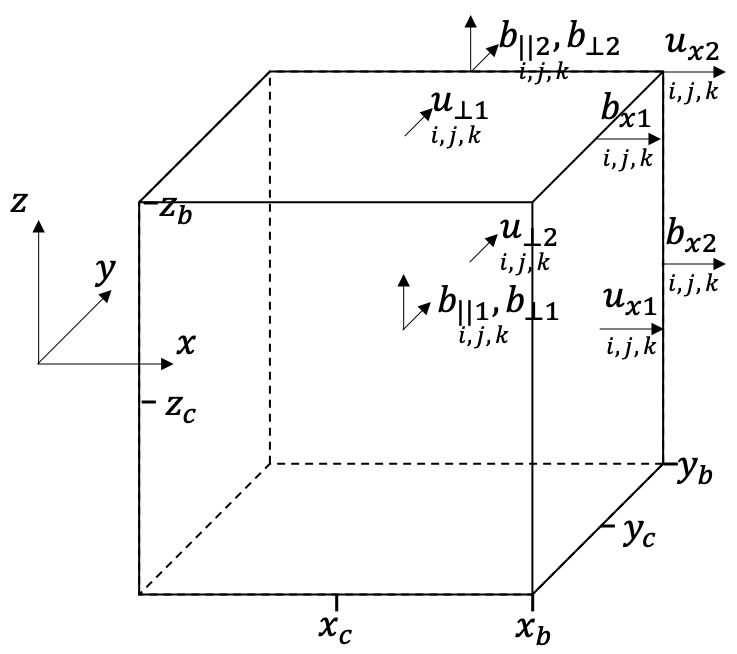
\includegraphics[width=0.6\textwidth]{grid2_.png}
    \caption{Diagram showing the location where every variable is defined for each cell.}
    \label{fig:grid}
\end{figure}

\begin{figure}[!htp]
    \centering
    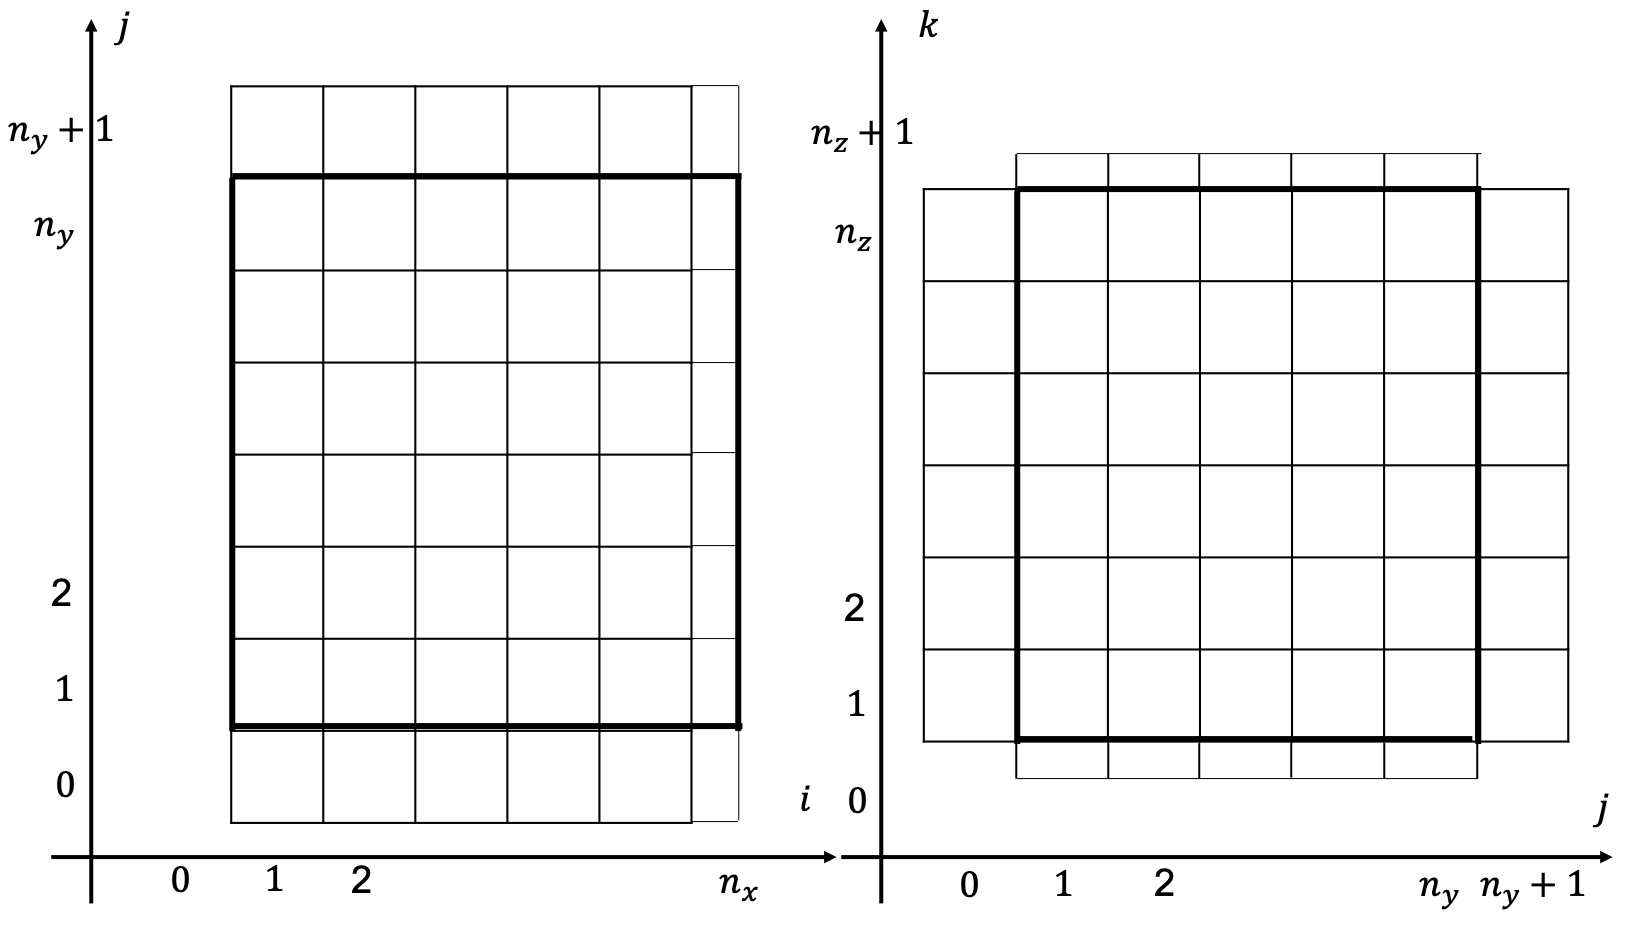
\includegraphics[width=0.9\textwidth]{grid2_2.png}
    \caption{Diagram of the physical and ghost domain. The thick line denotes the boundary between the physical and ghost domain.}
    \label{fig:grid2}
\end{figure}

We stagger the grid as illustrated in Figure \ref{fig:grid}. Hence, the MHD equations become:
\[\pdv{u_{x1}}{t}=\frac{1}{\rho}\left[\sin\alpha\pdv{b_{x2}}{y}+\cos\alpha\pdv{b_{x1}}{z} - \pdv{b_{||1}}{x}\right]\]
\[\pdv{u_{x2}}{t}=\frac{1}{\rho}\left[\sin\alpha\pdv{b_{x1}}{y}+\cos\alpha\pdv{b_{x2}}{z} - \pdv{b_{||2}}{x}\right]\]
\[\pdv{u_{\perp1}}{t}=\frac{1}{\rho}\left[\sin\alpha\pdv{b_{\perp2}}{y}+\cos\alpha\pdv{b_{\perp1}}{z}-\cos\alpha\pdv{b_{||2}}{y}+\sin\alpha\pdv{b_{||1}}{z}\right],\]
\[\pdv{u_{\perp2}}{t}=\frac{1}{\rho}\left[\sin\alpha\pdv{b_{\perp1}}{y}+\cos\alpha\pdv{b_{\perp2}}{z}-\cos\alpha\pdv{b_{||1}}{y}+\sin\alpha\pdv{b_{||2}}{z}\right],\]
\[\pdv{b_{x1}}{t}=\sin\alpha\pdv{u_{x2}}{y}+\cos\alpha\pdv{u_{x1}}{z},\]
\[\pdv{b_{x2}}{t}=\sin\alpha\pdv{u_{x1}}{y}+\cos\alpha\pdv{u_{x2}}{z},\]
\[\pdv{b_{\perp1}}{t}=\sin\alpha\pdv{u_{\perp2}}{y}+\cos\alpha\pdv{u_{\perp1}}{z},\]
\[\pdv{b_{\perp2}}{t}=\sin\alpha\pdv{u_{\perp1}}{y}+\cos\alpha\pdv{u_{\perp2}}{z},\]
\[\pdv{b_{||1}}{t}=-\left[\pdv{u_{x1}}{x}+\cos\alpha\pdv{u_{\perp2}}{y}-\sin\alpha\pdv{u_{\perp1}}{z}\right],\]
\[\pdv{b_{||2}}{t}=-\left[\pdv{u_{x2}}{x}+\cos\alpha\pdv{u_{\perp1}}{y}-\sin\alpha\pdv{u_{\perp2}}{z}\right].\]
Where:
\begin{itemize}
    \item $u_{x1}$ is defined at $(x_b,y_c,z_c)$.
    \item $u_{x2}$ is defined at $(x_b,y_b,z_b)$.
    \item $u_{\perp1}$ is defined at $(x_c,y_c,z_b)$.
    \item $u_{\perp2}$ is defined at $(x_c,y_b,z_c)$.
    \item $b_{x1}$ is defined at $(x_b,y_c,z_b)$.
    \item $b_{x2}$ is defined at $(x_b,y_b,z_c)$.
    \item $b_{\perp1}$ and $b_{||1}$ are defined at $(x_c,y_c,z_c)$.
    \item $b_{\perp2}$ and $b_{||2}$ are defined at $(x_c,y_b,z_b)$.
\end{itemize}

Figure \ref{fig:grid2} illustrates the number of cells used and how they are arranged. The physical domain is defined by
\begin{itemize}
    \item \texttt{xc(1:nx)},
    \item \texttt{xb(0:nx-1)},
    \item \texttt{yc(1:ny)},
    \item \texttt{yb(1:ny)},
    \item \texttt{zc(1:nz)},
    \item \texttt{zb(0:nz)},
\end{itemize}
the full computational domain, including ghost cells is given by
\begin{itemize}
    \item \texttt{xc(1:nx)},
    \item \texttt{xb(0:nx-1)},
    \item \texttt{yc(0:ny+1)},
    \item \texttt{yb(0:ny+1)},
    \item \texttt{zc(0:nz+1)},
    \item \texttt{zb(0:nz)},
\end{itemize}
where $b_x$, $b_{||}$ and $b_{\perp}$ do not have ghost cells in the $z$-direction because the velocity is set to zero at the boundaries.
% \begin{itemize}
%     \item \texttt{ux1(0:nx-1,1:ny,1:nz)},
%     \item \texttt{ux2(0:nx-1,1:ny,0:nz)},
%     \item \texttt{u$\perp$1(1:nx,1:ny,0:nz)},
%     \item \texttt{u$\perp$2(1:nx,1:ny,1:nz)},
%     \item \texttt{bx1(0:nx-1,1:ny,0:nz)},
%     \item \texttt{bx2(0:nx-1,1:ny,1:nz)},
%     \item \texttt{b||1(1:nx,1:ny,1:nz)},
%     \item \texttt{b||2(1:nx,1:ny,0:nz)},
%     \item \texttt{b$\perp$1(1:nx,1:ny,1:nz)},
%     \item \texttt{b$\perp$2(1:nx,1:ny,0:nz)}.
% \end{itemize}
% The computational domain with ghost cells is defined by
% \begin{itemize}
%     \item \texttt{ux1(0:nx-1,0:ny+1,0:nz+1)},
%     \item \texttt{ux2(0:nx-1,0:ny+1,0:nz)},
%     \item \texttt{u$\perp$1(1:nx,0:ny+1,0:nz)},
%     \item \texttt{u$\perp$2(1:nx,0:ny+1,0:nz+1)},
%     \item \texttt{bx1(0:nx-1,0:ny+1,0:nz)},
%     \item \texttt{bx2(0:nx-1,0:ny+1,1:nz)},
%     \item \texttt{b||1(1:nx,0:ny+1,1:nz)},
%     \item \texttt{b||2(1:nx,0:ny+1,0:nz)},
%     \item \texttt{b$\perp$1(1:nx,0:ny+1,1:nz)},
%     \item \texttt{b$\perp$2(1:nx,0:ny+1,0:nz)},
% \end{itemize}

\section*{Boundary conditions}

The physical domain is given by
\[0\le x\le L_x,\]
\[0\le y\le L_y\]
\[0 \le z \le L_z\]
The boundary conditions are:
\begin{itemize}
    \item At $x=0$ we impose
    \[u_x=b_x=0,\]
    this should ensure that
    \[\pdv{u_\perp}{x}=\pdv{b_\perp}{x}=\pdv{b_{||}}{x}=0,\]
    on the boundary.
    
    \item At $x=L_x$ we impose
    \[u_\perp=b_\perp=b_{||}=0\]
    this should ensure that
    \[\pdv{u_x}{x}=\pdv{b_x}{x}=0,\]
    on the boundary.
    
    \item At $y=0$ and $y=L_y$ periodic boundaries are imposed.
    \item At $z=0$ and $z=L_z$ we impose
    \[u_x=u_\perp=0.\]
    We also impose that the ghost flow must be the negative mirror image of the domain flow. No boundary conditions are imposed on the magnetic field directly.
    
\end{itemize}


\end{document}
